\documentclass{report}

% ==============================

% Configuration files for custom packages and macros
\input{config/preamble}
\input{config/macros}
\input{config/letterfonts}

% ==============================

\title{\Huge{COMP 458/558}\\Quantum Computing Algorithms}
\author{\huge{Micah Kepe}}
\date{}

\begin{document}

\maketitle
\newpage% or \cleardoublepage
\pdfbookmark[<level>]{<title>}{<dest>}
\pdfbookmark[section]{\contentsname}{toc}
\tableofcontents
\pagebreak

% ==============================
% PHASE I: INTRODUCTION
% ==============================
\chapter{Phase I: Introduction and Background}

% ● Overview of quantum computing concepts and
% applications
% ● Historical background and current state of quantum
% computing
% ● Review of linear algebra concepts, notation, and
% vector spaces
\section{Lecture 1: Overview of Quantum Computing Concepts}\label{sec:lecture1}
\dfn{Quantum Computing}{\textbf{Quantum computing} is a computational paradigm
  leveraging quantum mechanical principles such as superposition, entanglement,
  and interference to perform computations that can surpass the capabilities of
  classical systems for specific tasks.

  \footnote{Superposition \index{superposition} allows quantum bits (qubits)
    to exist in multiple states simultaneously, and entanglement enables
correlations between qubits even at a distance.}}

\subsection*{Historical Development of Quantum Computing}
\begin{itemize}
  \item \textbf{1980s-1990s:} Conception of quantum computing, with
    foundational ideas like the quantum Turing machine and quantum gates.

  \item \textbf{1990s-2000s:} Demonstration of key building blocks, such as
    quantum algorithms (e.g., Shor's and Grover's algorithms).

  \item \textbf{2016:} Emergence of quantum computing clouds, enabling
    access to quantum hardware via the internet.

  \item \textbf{2019:} First claims of \textbf{quantum advantage},
    showcasing tasks where quantum computers outperform classical
    counterparts.

  \item \textbf{2024:} Increasing qubit counts and improvements in quantum
    error correction techniques.

\end{itemize}

\subsection*{Applications of Quantum Computing}

Quantum computing offers \textbf{speedup} in areas such as:

\begin{enumerate}
  \item \textbf{Quantum Simulation:} Applications in chemistry, physics,
    and materials science, such as simulating molecular energy levels and
    drug discovery.

  \item \textbf{Security and Encryption:} Developing quantum-safe
    cryptographic protocols and random number generation.

  \item \textbf{Search and Optimization:} Enhancing solutions for weather
    forecasting, financial modeling, traffic planning, and resource
    allocation.

\end{enumerate}

\ex{Example: Quantum Speedup in Drug Discovery}{Drug discovery benefits from
  quantum simulation by enabling more accurate modeling of molecular
interactions, which classical computers struggle to achieve efficiently.}

\subsection*{Classical vs. Quantum Computing Paradigms}
\begin{itemize}

  \item \textbf{Classical Computing:\index{classical computing}} Utilizes
    traditional processing units (CPU, GPU, FPGA) and executes deterministic
    computations.

  \item \textbf{Quantum Computing:} Employs quantum processing units (QPU)
    with probabilistic computation based on quantum states.

\end{itemize}

\nt{Note: Classical computing paradigms still dominate in tasks that require
  precision and deterministic results. Quantum computing excels in
probabilistic or exponentially large state-space problems.}


\section{Lecture 2: Review of Linear Algebra Concepts}
\dfn{Vectors: Row and Column Vectors}{A \textbf{vector} is an ordered list of numbers, which can be represented as either a row or column vector. The components of vectors in quantum computing belong to the field of complex numbers ($\mathbb{C}$).}

\subsection*{Column Vectors}
A column vector is a vertical arrangement of numbers:
\[ \mathbf{v} = \begin{bmatrix} v_1 \\ v_2 \\ \vdots \\ v_n \end{bmatrix}, \quad v_i \in \mathbb{C}. \]

\subsection*{Row Vectors}
A row vector is the complex conjugate transpose (adjoint) of a column vector:
\[ \mathbf{v}^\dagger = \begin{bmatrix} \overline{v_1} & \overline{v_2} & \dots & \overline{v_n} \end{bmatrix}. \]

\dfn{Inner Product}{The \textbf{inner product} of two vectors $\mathbf{v}, \mathbf{w} \in \mathbb{C}^n$ is defined as:
\[ \langle \mathbf{v}, \mathbf{w} \rangle = \mathbf{v}^\dagger \mathbf{w} = \sum_{i=1}^n \overline{v_i}w_i. \]}

\ex{Example: Inner Product}{Let $\mathbf{v} = \begin{bmatrix} 1 + i \\ 2 \end{bmatrix}$ and $\mathbf{w} = \begin{bmatrix} 3 \\ i \end{bmatrix}$. Then:
\[ \langle \mathbf{v}, \mathbf{w} \rangle = (1 - i)(3) + (2)(i) = 3 - 3i + 2i = 3 - i. \]}

\dfn{Outer Product}{The \textbf{outer product} of two vectors $\mathbf{v} \in \mathbb{C}^m$ and $\mathbf{w} \in \mathbb{C}^n$ produces an $m \times n$ matrix:
\[ \mathbf{v}\mathbf{w}^\dagger = \begin{bmatrix} v_1 \\ v_2 \\ \vdots \\ v_m \end{bmatrix} \begin{bmatrix} \overline{w_1} & \overline{w_2} & \dots & \overline{w_n} \end{bmatrix}. \]}

\dfn{Orthogonality}{Two vectors $\mathbf{v}, \mathbf{w} \in \mathbb{C}^n$ are \textbf{orthogonal} if their inner product is zero:
\[ \langle \mathbf{v}, \mathbf{w} \rangle = 0. \]}

\ex{Example: Orthogonality}{Let $\mathbf{v} = \begin{bmatrix} 1 \\ i \end{bmatrix}$ and $\mathbf{w} = \begin{bmatrix} i \\ 1 \end{bmatrix}$. Then:
\[ \langle \mathbf{v}, \mathbf{w} \rangle = (1)(i) + (i)(1) = i - i = 0. \]}

\dfn{Eigenvalues and Eigenvectors}{For a square matrix $A \in \mathbb{C}^{n \times n}$, a vector $\mathbf{v} \neq \mathbf{0}$ is an \textbf{eigenvector} if:
\[ A\mathbf{v} = \lambda\mathbf{v}, \]
where $\lambda \in \mathbb{C}$ is the \textbf{eigenvalue}.}


%%%%

% ● Quantum state representation and quantum bits
% (qubits)
% ● Probability theory and its application to quantum
% systems
% ● Measurement and quantum state collapse
% ● Statistical analysis of quantum measurements
\section{Lecture 3: Quantum Bits and Quantum States}

\dfn{Qubit}{A \textbf{qubit} is the fundamental unit of quantum information. Unlike a classical bit, which is either $0$ or $1$, a qubit can exist in a \vocab{superposition} of states:
\[ |\psi\rangle = \alpha|0\rangle + \beta|1\rangle, \quad \text{where } \alpha, \beta \in \mathbb{C} \text{ and } |\alpha|^2 + |\beta|^2 = 1 \]

Key features of qubits include:
\begin{itemize}
    \ii \textbf{Superposition:} A qubit can exist simultaneously in multiple basis states.
    \ii \textbf{Complex Amplitudes:} Coefficients $\alpha$ and $\beta$ are complex numbers carrying magnitude and phase information.
    \ii \textbf{Interference:} Quantum states can interfere constructively or destructively.
    \ii \textbf{Entanglement:} Qubits can be correlated in ways that classical bits cannot.
\end{itemize}}

\dfn{Classical Computing Paradigms}{Quantum computing introduces a fundamentally different computational model:
\begin{itemize}
    \ii \textbf{Deterministic Computing:} Uses discrete states (0 or 1) with predictable transitions.
    \ii \textbf{Analog Computing:} Uses continuous values susceptible to noise accumulation.
    \ii \textbf{Probabilistic Computing:} Represents probabilistic mixtures of states.
    \ii \textbf{Quantum Computing:} Allows coherent superposition with complex amplitudes and quantum interference.
\end{itemize}}

\dfn{Dirac Notation}{Quantum states are represented using \vocab{Dirac notation} (bra-ket notation):
\begin{itemize}
    \ii \textbf{Ket:} \( |0\rangle, |1\rangle \) represent computational basis states
    \ii Computational basis vectors:
    \[
    |0\rangle = \begin{bmatrix} 1 \\ 0 \end{bmatrix}, \quad
    |1\rangle = \begin{bmatrix} 0 \\ 1 \end{bmatrix}
    \]
    \ii General state: \( |\psi\rangle = \alpha|0\rangle + \beta|1\rangle \)
\end{itemize}}

\dfn{Basis States}{Common qubit bases include:
\begin{itemize}
    \ii \textbf{Computational Basis:} \( |0\rangle, |1\rangle \)
    \ii \textbf{Hadamard Basis:}
    \[ |+\rangle = \frac{1}{\sqrt{2}}(|0\rangle + |1\rangle), \quad
       |-\rangle = \frac{1}{\sqrt{2}}(|0\rangle - |1\rangle) \]
    \ii \textbf{Circular Polarization Basis:}
    \[ |L\rangle = \frac{1}{\sqrt{2}}(|0\rangle + i|1\rangle), \quad
       |R\rangle = \frac{1}{\sqrt{2}}(|0\rangle - i|1\rangle) \]
\end{itemize}}

\dfn{Bloch Sphere}{A geometric representation of a single qubit state:
\[ |\psi\rangle = \cos\left(\frac{\theta}{2}\right)|0\rangle + e^{i\phi}\sin\left(\frac{\theta}{2}\right)|1\rangle \]
Where:
\begin{itemize}
    \ii \( \theta \in [0,\pi] \) is the polar angle
    \ii \( \phi \in [0, 2\pi) \) is the azimuthal angle
    \ii Cartesian coordinates:
    \[ x = \sin\theta \cos\phi, \quad
       y = \sin\theta \sin\phi, \quad
       z = \cos\theta \]
\end{itemize}}

\dfn{Quantum Measurement}{When a qubit is measured:
\begin{itemize}
    \ii The quantum state \textit{collapses} to an eigenstate
    \ii Measurement probability depends on squared amplitude
    \ii Computational basis measurement probabilities:
    \[ P(0) = |\alpha|^2, \quad P(1) = |\beta|^2 \]
    \ii Post-measurement state:
    \[ |\psi_{\text{new}}\rangle = \frac{|b\rangle \langle b | \psi \rangle}{\sqrt{P(b)}} \]
\end{itemize}}

\ex{Measurement Example}{For the state \( |\psi\rangle = \frac{1}{\sqrt{3}}|0\rangle + \sqrt{\frac{2}{3}}|1\rangle \):
\begin{itemize}
    \ii Probability of measuring \( |0\rangle \): \( P(0) = \frac{1}{3} \)
    \ii Probability of measuring \( |1\rangle \): \( P(1) = \frac{2}{3} \)
\end{itemize}}

\qs{Orthonormality Check}{Verify the inner products of basis states:
\begin{align*}
    \langle 0 | 1 \rangle &= 0 \\
    \langle 0 | 0 \rangle &= 1 \\
    \langle + | + \rangle &= 1 \\
    \langle + | - \rangle &= 0
\end{align*}}

\sol{These relations hold due to the orthonormal nature of quantum basis states.}



%%%%

% ● Quantum gates and transformations
% ● Unitary matrices and their properties
% ● Quantum circuits, systems, and properties
% ● Multi-qubit systems and entanglement
\section{Lecture 4: Quantum Gates and Transformations}

Quantum gates manipulate qubits through unitary transformations, preserving
quantum information and enabling quantum computation. This section explores
key quantum operations, their mathematical properties, and circuit
representations.

\dfn{Qubit Superposition and Hilbert Space}{A \textbf{qubit} exists in a
  complex vector space called a \textbf{Hilbert space}. The state of a qubit
  is given by:
  \[
    |\psi\rangle = \alpha |0\rangle + \beta |1\rangle, \quad \text{where }
    \alpha, \beta \in \mathbb{C} \text{ and } |\alpha|^2 + |\beta|^2 = 1.
  \]
}

\subsection*{Measurement and Superposition Collapse}

When a qubit is measured in the computational basis $\{|0\rangle,
|1\rangle\}$, it collapses to one of the basis states with probability:

\[
  \boxed{
    P(0) = \norm{\alpha_1}^2, \quad P(1) = \norm{\alpha_2}^2.
  }
\]

The post-measurement state is:

\[
  \boxed{
    |\psi_{\text{measurement}}\rangle = \frac{|b\rangle \langle b | \psi
    \rangle}{\sqrt{P(b)}}
  }
\]

\noindent
where $b \in \{0,1\}$. This formula captures the quantum measurement
postulate and ensures proper normalization of the post-measurement state.

\vspace{0.3cm}

In the computational basis, the probability of measuring $|b\rangle$ is:

\[
  \boxed{
    P(b) = \norm{\langle b | \psi \rangle}^2
  }
\]

\nt{Probability Properties of Measurement:
  \[
    \begin{aligned}
      P(0) &= 1 - P(1) \\
      P(+) &= 1 - P(-) \\
      P(+i) &= 1 - P(-i)
    \end{aligned}
  \]
}

\subsection*{Quantum Gates and Operations}

Quantum gates are unitary matrices that transform qubits. A general qubit
transformation is given by:

\[
  |\psi_{\text{final}}\rangle = U |\psi_{\text{initial}}\rangle
\]

\noindent
where $U$ is a unitary matrix satisfying $U^\dagger U = I$. Key properties of
quantum gates include:

\begin{itemize}
  \item \textbf{Reversibility:} All quantum operations are reversible due
    to unitarity
  \item \textbf{Preservation of Norm:} The normalization condition
    $|\alpha|^2 + |\beta|^2 = 1$ is preserved
  \item \textbf{Linearity:} Gates act linearly on superposition states
\end{itemize}

\dfn{Rotation Gates}{Rotation gates rotate a qubit state around the Bloch
  sphere:
  \begin{itemize}
    \item \textbf{Rotation about X-axis:}
      \[
        \boxed{
          R_X(\omega) =
          \begin{bmatrix}
            \cos\frac{\omega}{2} & -i\sin\frac{\omega}{2} \\
            -i\sin\frac{\omega}{2} & \cos\frac{\omega}{2}
          \end{bmatrix}
        }
      \]

      Effect: Rotates state by angle $\omega$ around X-axis

    \item \textbf{Rotation about Y-axis:}
      \[
        \boxed{
          R_Y(\omega) =
          \begin{bmatrix}
            \cos\frac{\omega}{2} & -\sin\frac{\omega}{2} \\
            \sin\frac{\omega}{2} & \cos\frac{\omega}{2}
          \end{bmatrix}
        }
      \]

      Effect: Rotates state by angle $\omega$ around Y-axis

    \item \textbf{Rotation about Z-axis:}
      \[
        \boxed{
          R_Z(\omega) =
          \begin{bmatrix}
            e^{-i\omega/2} & 0 \\
            0 & e^{i\omega/2}
          \end{bmatrix}
        }
      \]

      Effect: Adds a relative phase between $|0\rangle$ and $|1\rangle$
      components
  \end{itemize}
}

\dfn{Pauli Matrices and Gates}{The \textbf{Pauli matrices} define fundamental
  quantum operations:
  \begin{itemize}
    \item \textbf{Pauli-X (NOT Gate, Bit-Flip):}
      \[
        \boxed{
          X = \begin{bmatrix} 0 & 1 \\ 1 & 0 \end{bmatrix}
        }
      \]

      Effect: $X|0\rangle = |1\rangle$, $X|1\rangle = |0\rangle$

    \item \textbf{Pauli-Y (Combination of X and Z with phase):}
      \[
        \boxed{
          Y = \begin{bmatrix} 0 & -i \\ i & 0 \end{bmatrix}
        }
      \]

      Effect: $Y|0\rangle = i|1\rangle$, $Y|1\rangle = -i|0\rangle$

    \item \textbf{Pauli-Z (Phase-Flip Gate):}
      \[
        \boxed{
          Z = \begin{bmatrix} 1 & 0 \\ 0 & -1 \end{bmatrix}
        }
      \]

      Effect: $Z|0\rangle = |0\rangle$, $Z|1\rangle = -|1\rangle$

  \end{itemize}

  \aside{Each of these matrices is both \textbf{Hermitian} ($A = A^\dagger$) and
  \textbf{unitary} ($A^\dagger A = I$).}

  Important relationships:
  \begin{itemize}
    \item $X^2 = Y^2 = Z^2 = I$
    \item $XY = iZ$, $YZ = iX$, $ZX = iY$
    \item $YX = -iZ$, $ZY = -iX$, $XZ = -iY$
\end{itemize}}

\subsection*{Circuit Notation}
Quantum circuits visually represent quantum
  operations. Each qubit is represented as a horizontal line, and gates are
  applied sequentially from left to right. Important circuit elements include:
  \begin{itemize}
    \item \textbf{Single-qubit gates:} Represented as boxes with gate symbols
    \item \textbf{Measurements:} Depicted with a meter symbol
    \item \textbf{Time flow:} Left to right in circuits (\textbf{opposite of
      matrix multiplication order})
\end{itemize}

\ex{Example: Complex Circuit Analysis}{Consider the circuit applying the
  sequence $HZH$ to $|0\rangle$:
  \[
    \begin{aligned}
      |\psi_1\rangle &= H|0\rangle = \frac{1}{\sqrt{2}}(|0\rangle +
      |1\rangle) \\
      |\psi_2\rangle &= Z|\psi_1\rangle = \frac{1}{\sqrt{2}}(|0\rangle -
      |1\rangle) \\
      |\psi_3\rangle &= H|\psi_2\rangle = |1\rangle
    \end{aligned}
  \]

  This sequence performs a NOT operation on $|0\rangle$ using only Hadamard and
  Phase-flip gates.

  \[
    \begin{quantikz}
      \lstick{$|0\rangle$} & \gate{H} & \gate{Z} & \gate{H} & \one \\
    \end{quantikz}
  \]
}

\ex{Another Circuit Example}{
  \[
    \begin{aligned}
      XY \zero & = X \begin{bmatrix} 0 & -i \\ i & 0 \end{bmatrix} \begin{bmatrix} 1 \\ 0 \end{bmatrix}\\
      & = \begin{bmatrix} 0 & 1 \\ 1 & 0 \end{bmatrix} \begin{bmatrix} 0 \\ i \end{bmatrix} \\
      & = \begin{bmatrix} i \\ 0 \end{bmatrix} = i \one
    \end{aligned}
  \]

  \[
    \begin{quantikz}
      \lstick{$\zero$} & \gate{Y} & \gate{X} & i \zero \\
    \end{quantikz}
  \]
}

%%%%%%%%%%%%%%%%%%%%%%%

\qs{Exercise 1}{Apply the sequence $SXH$ to $|0\rangle$ and calculate:
  \begin{itemize}
    \item The final state vector
    \item The probabilities of measuring $|0\rangle$ and $|1\rangle$
    \item The possible post-measurement states
\end{itemize}}

\qs{Exercise 2}{Show that the Hadamard gate is its own inverse by calculating
$H^2$.}

\qs{Exercise 3}{Calculate the effect of applying $R_Z(\pi/2)$ to the state
$|+\rangle$.}

\sol{Exercise 1 Solution:
  \begin{align*}
    H|0\rangle &= \frac{1}{\sqrt{2}}(|0\rangle + |1\rangle) \\
    XH|0\rangle &= \frac{1}{\sqrt{2}}(|1\rangle + |0\rangle) =
    \frac{1}{\sqrt{2}}(|0\rangle + |1\rangle) \\
    SXH|0\rangle &= \frac{1}{\sqrt{2}}(|0\rangle + i|1\rangle)
  \end{align*}
  Therefore:
  \begin{itemize}
    \item Final state: $|\psi\rangle = \frac{1}{\sqrt{2}}(|0\rangle +
      i|1\rangle)$
    \item Measurement probabilities: $P(0) = P(1) = \frac{1}{2}$
    \item Post-measurement states: Either $|0\rangle$ or $|1\rangle$ with
      equal probability
\end{itemize}}


%%%%

% ● Reversibility property and no-cloning theorem
% ● Bell-state and GHZ state generation circuits
\section{Lecture 5: Other Quantum Gates, Measurement, Multi-Qubit Systems}

\dfn{Single-Qubit Gates}{Quantum gates manipulate individual qubits. Key
single-qubit gates include:}
\begin{itemize}
    \item \textbf{Hadamard Gate (H):}
    \[
        H = \frac{1}{\sqrt{2}} \begin{pmatrix} 1 & 1 \\ 1 & -1 \end{pmatrix}
    \]
    Creates superposition: \boxed{H\zero = \ket{+}, H\one = \ket{-}}

    Properties:
    \begin{itemize}
        \item Self-inverse: $H^2 = I$
        \item Maps computational basis to $\ket{\pm}$ basis:
        \begin{align*}
            \ket{+} &= \frac{1}{\sqrt{2}}(\zero + \one) \\
            \ket{-} &= \frac{1}{\sqrt{2}}(\zero - \one)
        \end{align*}
    \end{itemize}

    \item \textbf{Phase Gate (S):}
    \[
        S = \begin{pmatrix} 1 & 0 \\ 0 & i \end{pmatrix}
    \]
    Adds a $\pi/2$ phase to $\one$. Properties:
    \begin{itemize}
        \item Unitary but not Hermitian
        \item $S^2 = Z$
        \item Effect on $\ket{+}$ : \boxed{S\ket{+} =
          \frac{1}{\sqrt{2}}(\zero + i\one)}
    \end{itemize}

    \item \textbf{T Gate:}
    \[
        T = \begin{pmatrix} 1 & 0 \\ 0 & e^{i\pi/4} \end{pmatrix}
    \]
    Adds a $\pi/4$ phase to $\one$. Properties:
    \begin{itemize}
        \item $T^2 = S$
        \item $T^4 = Z$
        \item Often used in quantum error correction
    \end{itemize}

    \item \textbf{General Phase Gate } $P(\theta)$:
    \[
        P(\theta) = \begin{pmatrix} 1 & 0 \\ 0 & e^{i\theta} \end{pmatrix}
    \]
    Generalizes S and T gates: \boxed{S = P(\pi/2), T = P(\pi/4)}
\end{itemize}

\dfn{Important Relations}{
\begin{align*}
    Z &= H X H \\
    X &= H Z H
\end{align*}

Demonstrates duality between X and Z gates via Hadamard transformation.

Proof:
\[
HXH = \frac{1}{\sqrt{2}}\begin{pmatrix} 1 & 1 \\ 1 & -1 \end{pmatrix}
\begin{pmatrix} 0 & 1 \\ 1 & 0 \end{pmatrix}
\frac{1}{\sqrt{2}}\begin{pmatrix} 1 & 1 \\ 1 & -1 \end{pmatrix} =
\begin{pmatrix} 1 & 0 \\ 0 & -1 \end{pmatrix} = Z
\]
}

\dfn{Measurement}{Measurement collapses quantum states to basis states with
probabilities determined by amplitudes.}
\begin{itemize}
    \item \textbf{Z-basis:} Standard computational basis ($\zero$, $\one$)
        \begin{itemize}
            \item For state $\ket{\psi} = \alpha\zero + \beta\one$:
            \begin{align*}
                P(0) &= |\alpha|^2 \\
                P(1) &= |\beta|^2
            \end{align*}
        \end{itemize}
    \item \textbf{X-basis:} Hadamard basis ($\ket{+}$, $\ket{-}$)
      \begin{itemize}[label={*}]
            \item Measure in Z-basis after applying H gate
            \item $P(+) = |\bra{+}\psi\rangle|^2$
            \item $P(-) = |\bra{-}\psi\rangle|^2$
        \end{itemize}
    \item \textbf{Y-basis:} Eigenstates of Y
        \begin{itemize}
            \item $\ket{+i} = \frac{1}{\sqrt{2}}(\zero + i\one)$
            \item $\ket{-i} = \frac{1}{\sqrt{2}}(\zero - i\one)$
        \end{itemize}
\end{itemize}

\dfn{Multi-Qubit Systems}{States for multiple qubits are represented as
tensor products:}
\[
    \ket{\psi} = \sum_{x=0}^{2^n-1} \alpha_x \ket{x}, \quad \sum
    |\alpha_x|^2 = 1
\]

Properties of tensor products:
\begin{itemize}
    \item Not commutative: $(\ket{0} \otimes \ket{1} \neq \ket{1} \otimes
      \ket{0})$
    \item Associative: $((\ket{a} \otimes \ket{b}) \otimes \ket{c} = \ket{a}
      \otimes (\ket{b} \otimes \ket{c}))$
    \item Distributive: $((\alpha\ket{a} + \beta\ket{b}) \otimes \ket{c} =
      \alpha(\ket{a} \otimes \ket{c}) + \beta(\ket{b} \otimes \ket{c}))$
\end{itemize}

\vspace{0.3cm}

\ex{Example: Two-Qubit System}{
\[
    \ket{\psi} = \alpha_{00}\ket{00} + \alpha_{01}\ket{01} +
    \alpha_{10}\ket{10} + \alpha_{11}\ket{11}
\]
Bell state example:
\[
    \ket{\Phi^+} = \frac{1}{\sqrt{2}}(\ket{00} + \ket{11})
\]
This is a maximally entangled state.
}

\dfn{Circuit Diagrams}{Quantum circuits visually represent quantum operations
on qubits. They help to understand the sequence of quantum gates applied to
quantum states. The conventions are:}
\begin{itemize}
    \item Qubits are represented as horizontal lines (wires).
    \item Gates are shown as boxes or symbols on the wires.
    \item Time flows from left to right (the order of gate application).
    \item Measurement is depicted using a meter symbol.
    \item Classical information (post-measurement) is shown with double lines.
\end{itemize}

\subsubsection*{Single-Qubit Gate Example: Hadamard Gate}
\[
\begin{quantikz}
    \lstick{\ket{0}} & \gate{H} & \meter{}
\end{quantikz}
\]
This circuit applies the Hadamard gate $H$ to the state $\ket{0}$, creating
the superposition state $\frac{1}{\sqrt{2}}(\ket{0} + \ket{1})$, followed by
measurement.

\subsubsection*{Multi-Qubit System Example: CNOT Gate}
\[
\begin{quantikz}
    \lstick{\ket{0}} & \ctrl{1} & \qw \\
    \lstick{\ket{1}} & \targ{}  & \qw
\end{quantikz}
\]
This represents a controlled-NOT (CNOT) gate where the first qubit is the
control and the second is the target. If the control qubit is $\ket{1}$, the
target qubit flips; otherwise, it remains unchanged.

\subsubsection*{Bell State Preparation Circuit}
\[
\begin{quantikz}
    \lstick{\ket{0}} & \gate{H} & \ctrl{1} & \qw \\
    \lstick{\ket{0}} & \qw      & \targ{}  & \qw
\end{quantikz}
\]
This circuit prepares the Bell state $\ket{\Phi^+} = \frac{1}{\sqrt{2}}(\ket{00} + \ket{11})$. The first qubit undergoes a Hadamard gate, creating a superposition, followed by a CNOT gate that entangles the qubits.

\subsubsection*{Measurement in Different Bases}
\[
\begin{quantikz}
    \lstick{\ket{\psi}} & \gate{H} & \meter{} & \cw \\
    \lstick{\ket{\phi}} & \gate{S} & \meter{} & \cw
\end{quantikz}
\]

\begin{itemize}
  \item The first qubit is measured in the X-basis by applying a Hadamard
    gate before measurement.
  \item The second qubit undergoes a phase shift with the $S$ gate and is
    measured in the computational (Z) basis.
\end{itemize}

\vspace{0.3cm}

\subsection*{Exercises}
\qs{Exercise 1}{Prove that the Hadamard gate is unitary and Hermitian.}

\qs{Exercise 2}{For $\ket{\psi} = \frac{1}{\sqrt{2}}(\ket{00} + \ket{11})$,
find measurement probabilities for $\ket{00}$ and $\ket{11}$.}

\qs{Exercise 3}{Determine if $U = \frac{1}{\sqrt{2}}\begin{pmatrix} 1 & i \\
 i & 1 \end{pmatrix}$ is unitary.}

\qs{Exercise 4}{If we apply H $\otimes$ H to $\ket{00}$, what state do we get?}

\sol{Exercise 1 Solution:
To prove H is unitary and Hermitian:
\begin{align*}
    H^\dagger &= \frac{1}{\sqrt{2}}\begin{pmatrix} 1 & 1 \\ 1 & -1 \end{pmatrix} = H \\
    HH &= \frac{1}{2}\begin{pmatrix} 1 & 1 \\ 1 & -1 \end{pmatrix}\begin{pmatrix} 1 & 1 \\ 1 & -1 \end{pmatrix} = \begin{pmatrix} 1 & 0 \\ 0 & 1 \end{pmatrix} = I
\end{align*}
Thus, H is both unitary ($HH^\dagger = I$) and Hermitian ($H = H^\dagger$).}

\vspace{0.3cm}

\sol{Exercise 2 Solution:
For $\ket{\psi} = \frac{1}{\sqrt{2}}(\ket{00} + \ket{11})$:
\begin{align*}
    P(00) &= |\bra{00}\psi\rangle|^2 = \left|\frac{1}{\sqrt{2}}\right|^2 = \frac{1}{2} \\
    P(11) &= |\bra{11}\psi\rangle|^2 = \left|\frac{1}{\sqrt{2}}\right|^2 = \frac{1}{2}
\end{align*}
}

\vspace{0.3cm}

\sol{Exercise 3 Solution:
To verify unitarity, compute $UU^\dagger$:
\begin{align*}
    U^\dagger &= \frac{1}{\sqrt{2}}\begin{pmatrix} 1 & -i \\ -i & 1 \end{pmatrix} \\
    UU^\dagger &= \frac{1}{2}\begin{pmatrix} 1 & i \\ i & 1 \end{pmatrix}\begin{pmatrix} 1 & -i \\ -i & 1 \end{pmatrix} = \begin{pmatrix} 1 & 0 \\ 0 & 1 \end{pmatrix}
\end{align*}
Therefore, U is unitary.}

\vspace{0.3cm}

\sol{Exercise 4 Solution:
\begin{align*}
    (H \otimes H)\ket{00} &= (H\ket{0}) \otimes (H\ket{0}) \\
    &= \frac{1}{\sqrt{2}}(\ket{0} + \ket{1}) \otimes \frac{1}{\sqrt{2}}(\ket{0} + \ket{1}) \\
    &= \frac{1}{2}(\ket{00} + \ket{01} + \ket{10} + \ket{11})
\end{align*}
This creates an equal superposition of all two-qubit basis states.}

\section{Lecture 6: Multi-Qubit Gates and Circuit Construction}

$n$-qubit gates are unitary transformations that operate on $n$ qubits. This
section explores key multi-qubit gates, their properties, and how to
construct quantum circuits using these gates.

\subsection*{Controlled Gates}

\dfn{Controlled X Gate}{(CNOT) is a two-qubit gate that flips the target qubit
  if the control qubit is in state $\ket{1}$, and does nothing if the control
  qubit is in state $\ket{0}$. The matrix representation of CNOT is given by:

  \[
    CNOT = CX = \begin{pmatrix}
      1 & 0 & 0 & 0 \\
      0 & 1 & 0 & 0 \\
      0 & 0 & 0 & 1 \\
      0 & 0 & 1 & 0
    \end{pmatrix}
  \]

  Representing the gate in a circuit diagram:

  \begin{align*}
    \begin{quantikz}
      \lstick{$\ket{c}$} & \ctrl{1} & \qw \\
      \lstick{$\ket{t}$} & \gate{X} & \qw \\
    \end{quantikz}
  \end{align*}

  The control qubit is denoted by $\ket{c}$ and the target qubit is denoted by
$\ket{t}$.}

\vspace{0.3cm}

Applying the CNOT gate to a two-qubit state $\ket{\psi} = \alpha\ket{00} +
\beta\ket{01} + \gamma\ket{10} + \delta\ket{11}$:

\begin{equation}
  \begin{aligned}
      % CX |00>
    CX \ket{00} & = \begin{bmatrix}
      1 & 0 & 0 & 0 \\
      0 & 1 & 0 & 0 \\
      0 & 0 & 0 & 1 \\
      0 & 0 & 1 & 0
      \end{bmatrix} \begin{bmatrix}
      1 \\ 0 \\ 0 \\ 0
      \end{bmatrix} & = \begin{bmatrix}
      1 \\ 0 \\ 0 \\ 0
    \end{bmatrix} = \ket{00} \\
      % CX |01>
    CX \ket{01} & = \begin{bmatrix}
      1 & 0 & 0 & 0 \\
      0 & 1 & 0 & 0 \\
      0 & 0 & 0 & 1 \\
      0 & 0 & 1 & 0
      \end{bmatrix} \begin{bmatrix}
      0 \\ 1 \\ 0 \\ 0
      \end{bmatrix} & = \begin{bmatrix}
      0 \\ 1 \\ 0 \\ 0
    \end{bmatrix} = \ket{01} \\
      % CX |10>
    CX \ket{10} & = \begin{bmatrix}
      1 & 0 & 0 & 0 \\
      0 & 1 & 0 & 0 \\
      0 & 0 & 0 & 1 \\
      0 & 0 & 1 & 0
      \end{bmatrix} \begin{bmatrix}
      0 \\ 0 \\ 1 \\ 0
      \end{bmatrix} & = \begin{bmatrix}
      0 \\ 0 \\ 0 \\ 1
    \end{bmatrix} = \ket{11} \\
      % CX |11>
    CX \ket{11} & = \begin{bmatrix}
      1 & 0 & 0 & 0 \\
      0 & 1 & 0 & 0 \\
      0 & 0 & 0 & 1 \\
      0 & 0 & 1 & 0
      \end{bmatrix} \begin{bmatrix}
      0 \\ 0 \\ 0 \\ 1
      \end{bmatrix} & = \begin{bmatrix}
      0 \\ 0 \\ 1 \\ 0
    \end{bmatrix} = \ket{10}
  \end{aligned}
\end{equation}

\subsection*{Swapping Control and Target}

The control and target qubits of a CNOT gate can be swapped using Hadamard
gates:

\[
  (H \otimes H) \cdot CNOT_{\text{control,target}} \cdot (H \otimes H) =
  CNOT_{\text{target,control}}
\]

This transformation can be visualized in a circuit diagram:

\begin{align*}
  \begin{quantikz}
    \lstick{$\ket{c}$} & \gate{H} & \ctrl{1} & \gate{H} & \qw \\
    \lstick{$\ket{t}$} & \gate{H} & \gate{X} & \gate{H} & \qw \\
  \end{quantikz}
\end{align*}

\subsection*{SWAP Gate}

\dfn{SWAP Gate}{exchanges the states of two qubits. Its matrix representation
  is:

  \[
    SWAP = \begin{pmatrix}
      1 & 0 & 0 & 0 \\
      0 & 0 & 1 & 0 \\
      0 & 1 & 0 & 0 \\
      0 & 0 & 0 & 1
    \end{pmatrix}
  \]

  The action of SWAP on basis states is given by:

  \[
    SWAP\ket{ab} = \ket{ba}, \quad a,b \in \{0,1\}
  \]
}

\subsection*{Controlled-Z Gate}

\dfn{Controlled-Z Gate}{(CZ) applies a phase flip if both qubits are in state
  $\ket{1}$:

  \[
    CZ = \begin{pmatrix}
      1 & 0 & 0 & 0 \\
      0 & 1 & 0 & 0 \\
      0 & 0 & 1 & 0 \\
      0 & 0 & 0 & -1
    \end{pmatrix}
  \]
}

\subsection*{Toffoli Gate}

\dfn{Toffoli Gate}{(CCX) is a three-qubit gate with two control qubits and
  one target qubit. Its matrix representation is:

  \[
    Toffoli = \begin{pmatrix}
      1 & 0 & 0 & 0 & 0 & 0 & 0 & 0 \\
      0 & 1 & 0 & 0 & 0 & 0 & 0 & 0 \\
      0 & 0 & 1 & 0 & 0 & 0 & 0 & 0 \\
      0 & 0 & 0 & 1 & 0 & 0 & 0 & 0 \\
      0 & 0 & 0 & 0 & 1 & 0 & 0 & 0 \\
      0 & 0 & 0 & 0 & 0 & 1 & 0 & 0 \\
      0 & 0 & 0 & 0 & 0 & 0 & 0 & 1 \\
      0 & 0 & 0 & 0 & 0 & 0 & 1 & 0
    \end{pmatrix}
  \]

  The Toffoli gate is Hermitian and only flips the target qubit if both control
  qubits are in state $\ket{1}$.
}

\subsection*{Circuit Representations}

The standard circuit representations for these multi-qubit gates are:

\begin{align*}
  \begin{quantikz}
    % CNOT
    \lstick{CNOT:} & \ctrl{1} & \qw \\
    & \targ{} & \qw \\[0.5cm]
    % SWAP
    \lstick{SWAP:} & \swap{1} & \qw \\
    & \targX{} & \qw \\[0.5cm]
    % CZ
    \lstick{CZ:} & \ctrl{1} & \qw \\
    & \gate{Z} & \qw \\[0.5cm]
    % Toffoli
    \lstick{Toffoli:} & \ctrl{1} & \qw \\
    & \ctrl{1} & \qw \\
    & \targ{} & \qw
  \end{quantikz}
\end{align*}

\subsection*{Tensor Product Ordering and Circuit Representations}

When converting quantum circuits to mathematical expressions, it's important
to understand that tensor products are not commutative: $A \otimes B \neq B
\otimes A$ in general. However, we can modify the ordering of tensor products
in our mathematical representation as long as we maintain the dependencies
established by the circuit diagram. This leads to multiple valid mathematical
representations of the same quantum circuit.

\dfn{Bit Ordering Convention}{Due to the non-commutativity of tensor
  products, we adopt the convention of representing qubits from most
  significant to least significant in our mathematical expressions. For an
  $n$-qubit system:

  \[
  \ket{q_{n-1}q_{n-2}...q_1q_0} = \ket{q_{n-1}} \otimes \ket{q_{n-2}} \otimes
  ... \otimes \ket{q_1} \otimes \ket{q_0}
  \]

  where $q_0$ is the least significant qubit.
}

\noindent
For example, consider a circuit with two Hadamard gates applied to different
qubits:

\begin{align*}
  \begin{quantikz}
    \lstick{$\ket{q_1}$} & \gate{H} & \qw \\
    \lstick{$\ket{q_0}$} & \gate{H} & \qw
  \end{quantikz}
\end{align*}

This circuit can be represented mathematically in equivalent ways:

\[
  (H \otimes H)\ket{q_1q_0} = (H\ket{q_1}) \otimes (H\ket{q_0}) = H\ket{q_1}
  \otimes H\ket{q_0}
\]

\noindent
When gates have dependencies (like controlled operations), the ordering must
respect these dependencies. For the CNOT gate:

\begin{align*}
  \begin{quantikz}
    \lstick{$\ket{q_1}$} & \ctrl{1} & \qw \\
    \lstick{$\ket{q_0}$} & \gate{X} & \qw
  \end{quantikz}
\end{align*}

\noindent
The mathematical representation must preserve the control-target
relationship, though intermediate calculations may use different but
equivalent orderings:

\[
  CNOT_{1,0}\ket{q_1q_0} = CNOT(\ket{q_1} \otimes \ket{q_0})
\]

This flexibility in representation, while maintaining functional equivalence,
is particularly useful when analyzing complex quantum circuits or optimizing
quantum computations.


% ==============================
% PHASE II: FUNDAMENTALS
% ==============================
\chapter{Phase II: Fundamentals of Quantum Algorithms}

% ● Basic quantum algorithms
% ● Quantum computing using Cirq
\section{Lecture 7: Basic Quantum Algorithms and Computing Using \texttt{Circ} }\label{sec:Lecture 7} % (fold)

% section Lecture 7 (end)


% ● Grover's search algorithm and coding
% \section{Lecture 8: Entanglement, Bell State, and Intro to \texttt{Cirq}}
\label{sec:lecture8}

\subsection*{Review from Previous Lecture}

\qs{Quantum Circuit Final State}{
  Given this circuit diagram and assuming an initial state $\ket{\psi_i}
  =\ket{00}$, what will the final state $\ket{\psi_f}$ measure?

  \[
    \begin{quantikz}
      q_1 \quad \lstick{$\zero$} & \ctrl{0} & \gate{X} & \ctrl{1} & \swap{1}
                                 & \gate{H} & \meter{} \\
      q_0 \quad \lstick{$\zero$} & \ctrl{0} & \qw & \gate{X} & \swap{-1} &
      \gate{H} & \meter{} \\
    \end{quantikz}
  \]
}

\sol{\boxed{\ket{\psi_f} = \ket{--}}}

%%%%%%%%%%%%%%%

\index{entanglement}
\subsection*{Entanglement}

In this section, we introduce quantum entanglement—a phenomenon where the
states of two or more qubits become inseparably linked, leading to
correlations between measurement outcomes that cannot be explained classically.

\subsubsection*{What is Entanglement?}

To understand quantum entanglement, let's compare classical and quantum
communication systems:

\vspace{0.3cm}

\noindent
Consider two \textbf{classical} email clients, Alice and
Bob:

\begin{itemize}
  \item When Alice sends an email, she knows exactly what she sent
  \item Bob knows exactly what he received
  \item The message state is definite and independent
  \item Multiple copies can exist
\end{itemize}

\vspace{0.3cm}

\noindent
Now consider two \textbf{quantum} "email clients" with entangled qubits:

\begin{itemize}
  \item Neither Alice nor Bob knows their qubit's state before measurement
  \item When Alice measures her qubit, Bob's qubit instantly becomes correlated
  \item The qubits share a single quantum state
  \item No copies can be made (no-cloning theorem)
  \item The correlation exists regardless of distance
\end{itemize}

\vspace{0.3cm}

This "spooky action at a distance"\footnote{\href{https://en.wikipedia.org/wiki/Action\_at\_a\_distance\#\%22Spooky\_action\_at\_a\_distance\%22}{"Spooky action at a distance": \texttt{https://en.wikipedia.org/wiki/Action\_at\_a\_distance}}},
as Einstein called it, has no classical analog and is a fundamental feature
of quantum mechanics.

\index{entanglement!Bell state}
\subsubsection*{Bell-Pair Circuit}

The Bell-Pair circuit is the most analogous thing to quantum computing's
\texttt{Hello, world!} program. It prepares a maximally entangled two-qubit
state (a Bell state).


\[
  \begin{quantikz}
    q_1 \quad \lstick{$\zero$} & \gate{H} & \ctrl{1} & \meter{} \\
    q_0 \quad \lstick{$\zero$} & \qw & \gate{X} & \qw \\
  \end{quantikz}
\]


\index{entanglement!proof@\textit{proof}}
\begin{proof}{Showing Full Entanglement Mathematically}
  Starting with the initial state:

  \[
    \ket{\psi_0} = \ket{0}_1 \otimes \ket{0}_0 = \ket{00},
  \]

  we first apply a Hadamard gate on qubit \(q_1\):

  \[
    H\ket{0} = \frac{1}{\sqrt{2}}(\ket{0} + \ket{1}).
  \]

  Thus, the state after the Hadamard becomes:

  \[
    (H \otimes I)\ket{00} = \frac{1}{\sqrt{2}}(\ket{0} + \ket{1}) \otimes
    \ket{0} = \frac{1}{\sqrt{2}}(\ket{00} + \ket{10}).
  \]

  Next, we apply the CNOT gate with qubit \(q_1\) as the control and qubit
  \(q_0\) as the target. The CNOT gate acts as follows:

  \[
    \text{CNOT}\,\ket{00} = \ket{00}, \quad \text{CNOT}\,\ket{10} = \ket{11}.
  \]

  Thus, the final state after the CNOT is:

  \[
    \ket{\psi_{\text{Bell}}} = \frac{1}{\sqrt{2}}(\ket{00} + \ket{11}).
  \]

  This state is fully entangled since it cannot be factored as a tensor
  product of individual qubit states.

  \[
    \begin{quantikz}[column sep=0.5cm]
    & \gate{H} &
    \ctrl{1}\gategroup[2,steps=3,style={dashed,rounded
    corners,fill=blue!20, inner xsep=2pt},background,label style={label
    position=below,anchor=north,yshift=-0.2cm}]{{\sc Bell-Pair Creation}}
    & \qw & \qw \\
    & \qw & \gate{X} & \qw & \qw
    \end{quantikz}
  \]

\end{proof}

As a consequence of being fully entangled:

\begin{enumerate}
  \item Entangled circuits cannot be expressed as a product state. For
    example, the Bell state

    \[
      \ket{\psi_{\text{Bell}}} = \frac{1}{\sqrt{2}}(\ket{00} + \ket{11})
    \]

    cannot be decomposed into \(\ket{\phi}_1 \otimes \ket{\chi}_0\).

  \item Measurement outcomes are correlated. For instance, if qubit \(q_1\)
    is measured as \(\ket{0}\), then qubit \(q_0\) will also be found in the
    state \(\ket{0}\); similarly, if \(q_1\) is measured as \(\ket{1}\), then
    \(q_0\) will be \(\ket{1}\).

\end{enumerate}


\index{entanglement!n-qubit Bell state}
\subsubsection*{Extending the Bell-Pair Circuit to a $n$-Qubit System}

The Bell state can be generalized to an \(n\)-qubit system, often taking the
form of a Greenberger–Horne–Zeilinger (GHZ) state:

\index{entanglement!GHZ state}

\[
  \begin{quantikz}
    q_{n - 1}\quad \lstick{$\zero$} & \gate{H} & \ctrl{1} & \qw & \qw & \qw \\
    q_{n -2} \quad \lstick{$\zero$} & \qw & \gate{X} & \ctrl{0} & \qw & \qw \\
    \vdots \\
    q_{1} \quad \lstick{$\zero$} & \qw & \qw & \qw & \gate{X} & \ctrl{1} \\
    q_{0} \quad \lstick{$\zero$} & \qw & \qw & \qw & \qw & \gate{X} \\
  \end{quantikz}
\]


The $n$-qubit Bell circuit follows a clear pattern:

\begin{enumerate}
  \item Initial Hadamard gate on the topmost qubit creates superposition
  \item Cascade of CNOT gates propagates the entanglement down
  \item Each CNOT uses the previous qubit as control and current qubit as
    target
  \item Final state has all qubits entangled together
\end{enumerate}

The resulting state:

\[
  \boxed{
    \ket{\psi_f} = \frac{1}{\sqrt{2}}\lt(\ket{00\cdots 00} +
    \ket{11\cdots11}\rt)
  }
\]

represents a superposition where all qubits are either all 0 or all 1.
Measuring any qubit collapses the entire state, forcing all other qubits to
match the measured value.

\vspace{0.3cm}

It is important to note that there are equivalent diagrams that can be drawn for
the $n$-qubit Bell state circuit, and that you should not be fooled by diagrams
that do not match the general diagram shown above.


\ex{Alternative $n$-Qubit Bell Circuit}{

  \[
    \begin{quantikz}
      q_{n-1} \quad \lstick{$\zero$} & \gate{H} & \ctrl{1} & \ctrl{2} &
      \ctrl{3} & \qw \\
      q_{n-2} \quad \lstick{$\zero$} & \qw & \gate{X} & \qw & \qw & \qw \\
      q_{1} \quad \lstick{$\zero$} & \qw & \qw & \gate{X} & \qw & \qw \\
      q_{0} \quad \lstick{$\zero$} & \qw & \qw & \qw & \gate{X} & \qw
    \end{quantikz}
  \]

  This alternative representation achieves the same final state by having the
  first qubit control all CNOT operations directly. While functionally
  equivalent, this requires longer-range interactions which may be harder to
  implement on real quantum hardware.
}


\aside{Shorthand Notation Used for Final Quantum States\\
  Common notational shortcuts can be confusing for beginners. Here are some
  important distinctions:

  \begin{itemize}
    \item $\ket{+1}$ typically means $\frac{1}{\sqrt{2}}(\ket{01} +
      \ket{11})$, not $\ket{+} \otimes \ket{1}$

    \item $\ket{-1}$ represents $\frac{1}{\sqrt{2}}(\ket{01} - \ket{11})$,
      not to be confused with $-\ket{1}$ or $Z\ket{1}$

    \item In general, $\ket{\pm x}$ represents $\frac{1}{\sqrt{2}}(\ket{0x}
      \pm \ket{1x})$ where $x$ is a bit string

    \item The notation $\ket{\psi^+}$ and $\ket{\psi^-}$ is often used for
      Bell states $\frac{1}{\sqrt{2}}(\ket{01} \pm \ket{10})$
  \end{itemize}

  Always check the context and definitions when encountering shorthand
  notation, as conventions may vary between sources.
}

\index{entanglement!partial entanglement}
\paragraph{Partial Entanglement}

There also exists the middle ground of partially-entangled systems where only
some of the qubits are entangled while others have independent states.

\[
  \begin{quantikz}
    q_2 \quad \lstick{$\zero$} & \gate{H} & \qw & \qw \\
    q_1 \quad \lstick{$\zero$} & \gate{H} & \ctrl{1} & \qw \\
    q_0 \quad \lstick{$\zero$} & \qw & \gate{X} & \qw
  \end{quantikz}
\]

In this case, \(q_1\) and \(q_0\) become entangled through the CNOT gate,
while \(q_2\) remains in a superposition state but independent of the other
qubits. The final state is:

\[
  \ket{\psi_f} = \frac{1}{\sqrt{2}}\ket{+}_2 \otimes
  \frac{1}{\sqrt{2}}(\ket{00}_{10} + \ket{11}_{10})
\]

%%%%%%%%%%%%%%%

\subsection*{Getting Started with \texttt{Cirq}}

\index{Cirq}
\texttt{Cirq}\footnote{\texttt{Cirq} documentation:
\url{https://quantumai.google/cirq}} is an open-source framework for
programming quantum computers, developed by Google Quantum AI. It provides
tools for creating, manipulating, and optimizing quantum circuits, as well as
simulating quantum computations.

\vspace{0.3cm}

\noindent
\textbf{
  Key features of \texttt{Cirq} include:
}

\begin{itemize}
  \item Native support for quantum gates and circuits
  \item Built-in quantum simulator
  \item Tools for noise modeling and error mitigation
  \item Integration with TensorFlow Quantum
\end{itemize}

\index{Cirq!introduction}
\subsubsection*{Overview and Installation}
Cirq allows you to work with qubits, gates, and operations to build circuits.
To begin, install \texttt{Cirq} in your Python environment:

\begin{minted}{python}
  !pip install --quiet cirq
\end{minted}

Then import the library:

\begin{minted}{python}
  import cirq
\end{minted}

\subsubsection*{Defining Qubits}
Cirq supports different types of qubits:
\begin{itemize}
  \item \textbf{NamedQubit}: Qubits with custom names.
  \item \textbf{LineQubit}: Qubits arranged in a linear array.
  \item \textbf{GridQubit}: Qubits arranged in a 2D grid.
\end{itemize}
For example, to create line qubits:
\begin{minted}{python}
  q0, q1, q2 = cirq.LineQubit.range(3)
\end{minted}

\subsubsection*{Gates and Operations}
In Cirq, a \emph{Gate} represents an abstract quantum operation, while an
\emph{Operation} is a gate applied to specific qubits.

\begin{itemize}
  \item Single-qubit gates: \texttt{cirq.X}, \texttt{cirq.H},
    \texttt{cirq.S}, etc.
  \item Two-qubit gates: \texttt{cirq.CNOT}, \texttt{cirq.CZ},
    \texttt{cirq.SWAP}, etc.
\end{itemize}

Example: Applying a Hadamard gate to qubit \(q0\) and a CNOT with \(q0\) as
control and \(q1\) as target:

\begin{minted}{python}
  circuit = cirq.Circuit()
  circuit.append(cirq.H(q0))
  circuit.append(cirq.CNOT(q0, q1))
\end{minted}

\subsubsection*{Circuits and Moments}
A \emph{Circuit} in Cirq is composed of \emph{Moments}—collections of
operations that occur simultaneously (on disjoint sets of qubits). When you
append operations, Cirq automatically schedules them into moments.

\subsubsection*{Simulation and Measurement}

Cirq provides a simulator to compute the resulting state vector or sample
measurement outcomes.

\begin{itemize}
  \item \texttt{simulate()}: Returns the final state vector.
  \item \texttt{run()}: Samples measurement outcomes.
\end{itemize}

\textbf{Example: Creating and Simulating a Bell State}
\begin{minted}{python}
  import cirq

  # Create two line qubits.
  q0, q1 = cirq.LineQubit.range(2)

  # Construct the Bell state circuit.
  bell_circuit = cirq.Circuit(
  cirq.H(q0),         # Create superposition on q0.
  cirq.CNOT(q0, q1)   # Entangle q0 with q1.
  )

  print("Bell Circuit:")
  print(bell_circuit)

  # Initialize the simulator.
  simulator = cirq.Simulator()

  # Simulate to obtain the final state vector.
  result = simulator.simulate(bell_circuit)
  print("Final state vector:")
  print(result.final_state_vector)

  # Add measurement and run the circuit.
  bell_circuit.append(cirq.measure(q0, q1, key='result'))
  samples = simulator.run(bell_circuit, repetitions=1024)
  print("Measurement histogram:")
  print(samples.histogram(key='result'))
\end{minted}

\subsubsection*{Advanced Topics in Cirq}

Cirq also supports:

\begin{itemize}

  \item \textbf{Parameter Sweeps}: Optimize variational algorithms using free
    parameters.

  \item \textbf{Unitary Access and Decomposition}: Retrieve matrix
    representations and decompose complex gates.

  \item \textbf{Transformers}: Automatically merge or re-schedule operations
    for hardware compatibility.

\end{itemize}

\textbf{Example: Sweeping a Parameter in an \(X\) Gate}
\begin{minted}{python}
  import sympy
  import matplotlib.pyplot as plt

  # Define a qubit.
  q = cirq.GridQubit(1, 1)

  # Create a circuit with an X gate raised to a symbolic exponent.
  circuit = cirq.Circuit(cirq.X(q) ** sympy.Symbol('t'),
  cirq.measure(q, key='m'))

  # Sweep the parameter 't' from 0 to 2.
  param_sweep = cirq.Linspace('t', start=0, stop=2, length=200)

  # Simulate the sweep.
  simulator = cirq.Simulator()
  trials = simulator.run_sweep(circuit, param_sweep, repetitions=1000)

  # Plot the frequency of measuring 1.
  x_data = [trial.params['t'] for trial in trials]
  y_data = [trial.histogram(key='m')[1] / 1000.0 for trial in trials]
  plt.scatter(x_data, y_data)
  plt.xlabel("Parameter t")
  plt.ylabel("Frequency of 1")
  plt.show()
\end{minted}

%%%%%%%%%%%%%%%%%%%%%%%%%%%%%%%%%%%%%%%%%%%%%%
% End of Lecture 8
%%%%%%%%%%%%%%%%%%%%%%%%%%%%%%%%%%%%%%%%%%%%%%

% \section{Lecture 9: Grover's Search Algorithm}\label{sec:lecture9}

%%%%%%%%%%%%%%%%%%%%%%%%%%%%%%%%%%%%%%%%%%%%%%%%%%
% Problem Statement
%%%%%%%%%%%%%%%%%%%%%%%%%%%%%%%%%%%%%%%%%%%%%%%%%%
\index{Grover's Search Algorithm!problem statement}
\subsection*{Problem Statement}

Given a bitstring \( x \in \{0, 1\}^n \) and a function

\[
  f(x) =
  \begin{cases}
    1, & \text{if } x \text{ is the marked (or winning) state}, \\
    0, & \text{otherwise},
  \end{cases}
\]

our goal is to find the unique (or one of the) \( x \) such that \( f(x)=1 \).

\vspace{0.3cm}

In plain terms, imagine you have an unsorted database of \( N = 2^n \) items,
and only one item is “special.” Classically, you must check each item one by
one (on average, \( O(2^n) \) trials) to find the special item. Grover's
algorithm, however, uses quantum amplitude amplification to solve this
problem in only \( O(\sqrt{2^n}) \) iterations—a quadratic speedup over
classical search.

%%%%%%%%%%%%%%%%%%%%%%%%%%%%%%%%%%%%%%%%%%%%%%%%%%
% Grover's Algorithm Circuit (General n-qubit Version)
%%%%%%%%%%%%%%%%%%%%%%%%%%%%%%%%%%%%%%%%%%%%%%%%%%

\index{Grover's Search Algorithm!circuit}
\subsection*{Grover's Algorithm Circuit}

The general structure of Grover's algorithm is as follows:

\begin{enumerate}
  \item \textbf{State Preparation:} Initialize all qubits in the state
    \(\ket{0}^{\otimes n}\) and apply \( H^{\otimes n} \) to create a uniform
    superposition:

    \[
      \ket{s} = H^{\otimes n} \ket{0}^{\otimes n} = \frac{1}{\sqrt{2^n}}
      \sum_{x \in \{0,1\}^n} \ket{x}.
    \]

  \item \textbf{Grover Iteration:} Repeat the following two steps
    approximately \(\sqrt{2^n}\) times:

    \begin{itemize}
      \item \textbf{Oracle \(O\):} Flip the phase of the marked state(s);
        that is, for every \( x \),

        \[
          O \ket{x} = (-1)^{f(x)} \ket{x}.
        \]

        For example, if the winning state is \(\ket{w}\), then
        \( O\ket{w} = -\ket{w} \).

      \item \textbf{Diffusion Operator \(D\):} Reflect all amplitudes about
        the average amplitude. This operator is given by

        \[
          D = 2\ket{s}\bra{s} - I.
        \]

        In practice, \( D \) is implemented as

        \[
          D = H^{\otimes n} \; X^{\otimes n} \; (CZ) \; X^{\otimes n} \;
          H^{\otimes n},
        \]

        where the \(CZ\) gate here represents a controlled phase flip on
        \(\ket{1}^{\otimes n}\) (for \(n>2\), this is a multi-controlled \(Z\)
        gate).
    \end{itemize}
\end{enumerate}

The high-level circuit for an \( n \)-qubit Grover algorithm is illustrated as:

\[
\begin{quantikz}
  \lstick{$q_{n - 1}$} & \gate{H} &  \gate[5]{\shortstack{$f(x)$ \\ Oracle}} & \qw & \gate[5]{\text{Diffusion Circuit}} & \meter{} \\
  \lstick{$q_{n - 2}$} & \gate{H} &  &  & & \meter{} \\
  \vdots & \vdots & & \vdots & & \vdots \\
  \lstick{$q_1$} & \gate{H} & &  & & \meter{} \\
  \lstick{$q_0$} & \gate{H} &  & & & \meter{}
\end{quantikz}
\]

\[
  \hspace{1.5cm}
  \underbrace{\hspace{6cm}}_{\text{Repeat } \sqrt{2^n} \text{ times}}
\]

%%%%%%%%%%%%%%%%%%%%%%%%%%%%%%%%%%%%%%%%%%%%%%%%%%
% Inversion About the Mean Diagram
%%%%%%%%%%%%%%%%%%%%%%%%%%%%%%%%%%%%%%%%%%%%%%%%%%
\subsection*{Inversion About the Mean}

The diffusion operator \( D \) reflects the amplitudes of all states about
the average amplitude. This process is often referred to as "inversion about
the mean." The following diagram illustrates this concept:

\begin{center}
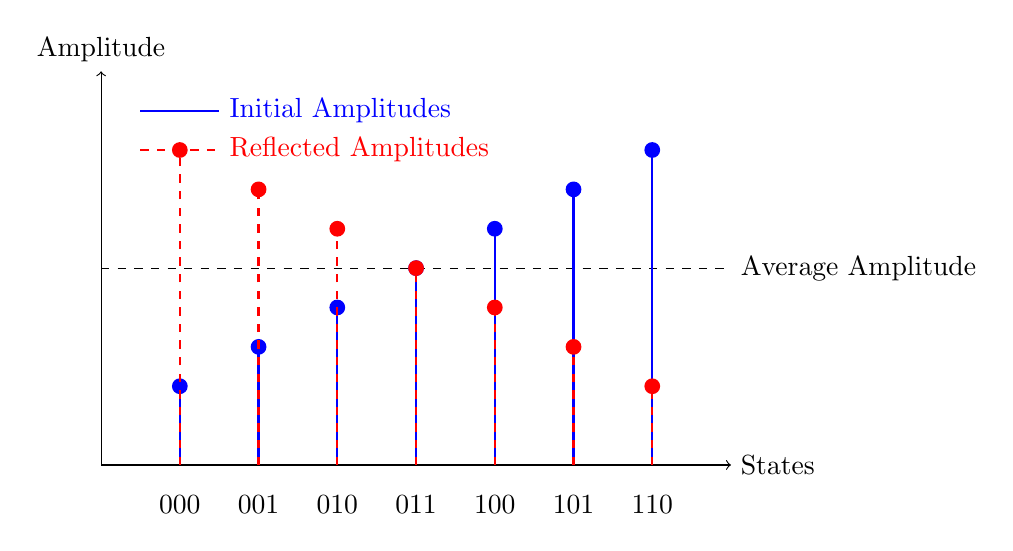
\begin{tikzpicture}
  % Draw axes
  \draw[->] (0,0) -- (8,0) node[right]{States};
  \draw[->] (0,0) -- (0,5) node[above]{Amplitude};

  % Draw average amplitude line
  \draw[dashed] (0,2.5) -- (8,2.5) node[right]{Average Amplitude};

  % Draw initial amplitudes
  \foreach \x/\y in {1/1, 2/1.5, 3/2, 4/2.5, 5/3, 6/3.5, 7/4} {
    \draw[blue, thick] (\x,0) -- (\x,\y);
    \fill[blue] (\x,\y) circle (0.1);
  }

  % Draw reflected amplitudes
  \foreach \x/\y in {1/4, 2/3.5, 3/3, 4/2.5, 5/2, 6/1.5, 7/1} {
    \draw[red, thick, dashed] (\x,0) -- (\x,\y);
    \fill[red] (\x,\y) circle (0.1);
  }

  % Labels
  \node at (1,-0.5) {\(\ket{000}\)};
  \node at (2,-0.5) {\(\ket{001}\)};
  \node at (3,-0.5) {\(\ket{010}\)};
  \node at (4,-0.5) {\(\ket{011}\)};
  \node at (5,-0.5) {\(\ket{100}\)};
  \node at (6,-0.5) {\(\ket{101}\)};
  \node at (7,-0.5) {\(\ket{110}\)};

  % Legend
  \draw[blue, thick] (0.5,4.5) -- (1.5,4.5) node[right]{Initial Amplitudes};
  \draw[red, thick, dashed] (0.5,4) -- (1.5,4) node[right]{Reflected Amplitudes};
\end{tikzpicture}
\end{center}

\vspace{0.3cm}

The blue bars represent the initial amplitudes of the states, and the red
dashed bars represent the amplitudes after inversion about the mean. The
marked state's amplitude is amplified, while the amplitudes of the other
states are reduced.


%%%%%%%%%%%%%%%%%%%%%%%%%%%%%%%%%%%%%%%%%%%%%%%%%%
% 2-Qubit Example
%%%%%%%%%%%%%%%%%%%%%%%%%%%%%%%%%%%%%%%%%%%%%%%%%%
\subsection*{2-Qubit Example}

To build intuition, consider the case \( n=2 \) (i.e., \( N=4 \)) with the winning
state chosen as \(\ket{11}\).

\vspace{0.3cm}

\textbf{Oracle:} For a 2-qubit system, the Oracle \(O\) can be implemented as a
controlled-\(Z\) (CZ) gate:
\[
  CZ =
  \begin{pmatrix}
    1 & 0 & 0 & 0 \\
    0 & 1 & 0 & 0 \\
    0 & 0 & 1 & 0 \\
    0 & 0 & 0 & -1
  \end{pmatrix},
\]

which multiplies the state \(\ket{11}\) by \(-1\).

\vspace{0.3cm}

\textbf{Diffusion Operator:} For 2 qubits, the diffusion operator is given by:

\[
  D = H^{\otimes 2}\; X^{\otimes 2}\; CZ\; X^{\otimes 2}\; H^{\otimes 2}.
\]

\vspace{0.3cm}

\textbf{2-Qubit Grover Circuit:}

\[
\begin{quantikz}
  \lstick{$\ket{0}$} & \gate{H} & \ctrl{1} & \gate{H} & \gate{X} & \qw & \ctrl{1} & \qw & \gate{X} & \gate{H} & \meter{} \\
  \lstick{$\ket{0}$} & \gate{H} & \ctrl{0} & \gate{H} & \gate{X} & \gate{H} & \gate{X} & \gate{H} & \gate{X} & \gate{H} & \meter{}
\end{quantikz}
\]

\vspace{0.3cm}

\noindent
\textbf{Explanation:}

\begin{itemize}
  \item \textbf{Oracle:} The Oracle adds a phase of \(-1\) to the winning
    state \(\ket{11}\), effectively marking it.
  \item \textbf{Diffusion Operator:} The diffusion circuit (implemented as
    \(H\;X\;CZ\;X\;H\)) reflects all amplitudes about the average. This
    inversion about the mean amplifies the amplitude of the marked state.
\end{itemize}

%%%%%%%%%%%%%%%%%%%%%%%%%%%%%%%%%%%%%%%%%%%%%%%%%%
% Algorithm Walkthrough and Pseudocode
%%%%%%%%%%%%%%%%%%%%%%%%%%%%%%%%%%%%%%%%%%%%%%%%%%

\index{Grover's Search Algorithm!pseudocode}
\subsection*{Walkthrough of the Algorithm and Generalization to \(n\) Qubits}

Grover's algorithm can be summarized in the following pseudocode:

\begin{algorithm}[H]
  \caption{Grover's Search Algorithm}
  \KwIn{A function \( f: \{0,1\}^n \rightarrow \{0,1\} \) with a unique
  marked state \( x_0 \) such that \( f(x_0) = 1 \).}
  \KwOut{The marked element \( x_0 \).}

  \textbf{Initialize:} Set the quantum state to \( \ket{\psi} \gets
  \ket{0}^{\otimes n} \).\\

  Apply \( H^{\otimes n} \) to obtain the uniform superposition:

  \[
    \ket{s} = H^{\otimes n}\ket{0}^{\otimes n} = \frac{1}{\sqrt{2^n}} \sum_{x
    \in \{0,1\}^n} \ket{x}.
  \]

  \For{\( i = 1 \) \KwTo \( \left\lfloor \frac{\pi}{4}\sqrt{2^n}
  \right\rfloor \)}{

    Apply the Oracle \( O \) which performs:

    \[
      O\ket{x} = (-1)^{f(x)}\ket{x},
    \]
    (i.e., flip the phase of the marked state).\;

    Apply the Diffusion Operator \( D = 2\ket{s}\bra{s} - I \)
    (which reflects amplitudes about the average).\;
  }

  Measure the state in the computational basis to obtain \( x_0 \).\;

\end{algorithm}

\vspace{0.3cm}

\noindent
\textbf{Detailed Explanation:}
\begin{enumerate}
  \item \textbf{Initialization:} All qubits are set to \(\ket{0}\) and then
    put into an equal superposition via \(H^{\otimes n}\).

  \item \textbf{Oracle Application:} The Oracle selectively flips the phase
    of the winning state(s) (e.g., for the marked state \(\ket{w}\),
    \(O\ket{w} = -\ket{w}\)).

  \item \textbf{Diffusion (Inversion about the Mean):} This operator reflects
    the state vector about the average amplitude. Geometrically, one can
    view the process as a rotation in a two-dimensional subspace.

  \item \textbf{Iteration:} Repeating the Oracle and Diffusion steps
    approximately \( \sqrt{2^n} \) times amplifies the probability amplitude of
    the marked state.

  \item \textbf{Measurement:} Finally, a measurement in the computational
    basis yields the marked element with high probability.
\end{enumerate}

This algorithm demonstrates how quantum algorithms can achieve a quadratic
speedup over classical brute-force search methods.

%%%%%%%%%%%%%%%%%%%%%%%%%%%%%%%%%%%%%%%%%%%%%%%%%%
% End of Lecture 9
%%%%%%%%%%%%%%%%%%%%%%%%%%%%%%%%%%%%%%%%%%%%%%%%%%


% ● Introduction to variational quantum algorithms
% ● Training and optimization of variational algorithms
% \section{Lecture 10: Quantum Logic Gates, Applying Grover's Search Algorithm
to SAT}\label{sec:lecture10}

%%%%%%%%%%%%%%

\subsection*{Review Question from Last Lecture}

\qs{Function of the Hadamard Layer in Grover's Algorithm}{
  Why does Grover's algorithm apply a Hadamard ($H$) gate to each of the $n$
  qubits at the beginning of the circuit?
}

\sol{
  The purpose of the Hadamard layer is that it allows up to work with all
  bitstring permutations simultaneously by putting all states in equal
  superposition.

  The Hadamard layer initializes the system in a uniform superposition of all
  possible $2^n$ states, allowing Grover's algorithm to explore all bitstring
  permutations simultaneously. For $n$ qubits starting at $|0\rangle^{\otimes
  n}$, applying $H^{\otimes n}$ yields:
  \[
    |s\rangle = H^{\otimes n} |0\rangle^{\otimes n} = \frac{1}{\sqrt{2^n}}
    \sum_{x \in \{0,1\}^n} |x\rangle.
  \]

  This equal superposition ensures that the algorithm can amplify the
  amplitude of the solution state(s) efficiently.
}

%%%%%%%%%%%%%

\subsection*{Quantum Implementations of Classical Logic Gates}

\index{quantum gates!OR gate}
\subsubsection*{OR Gate}

The quantum OR gate computes $c = a \lor b$ using a combination of CNOT and
Toffoli gates. Below is the two-way OR implementation:
\[
  \begin{quantikz}
    \lstick{$|a\rangle$} & \ctrl{1} & \ctrl{2} & \qw \\
    \lstick{$|b\rangle$} & \ctrl{1} & \targ{} & \qw \\
    \lstick{$|c\rangle$} & \targ{} & \targ{} & \qw
  \end{quantikz}
\]

\textbf{Truth Table:}
\[
  \begin{array}{ccc|c}
    a & b & c_{\text{in}} & c_{\text{out}} = a \lor b \\
    \hline
    0 & 0 & 0 & 0 \\
    0 & 1 & 0 & 1 \\
    1 & 0 & 0 & 1 \\
    1 & 1 & 0 & 1 \\
  \end{array}
\]

The circuit uses CCNOT (Toffoli) to set $c$ if both $a$ and $b$ are 1, then
CNOTs to flip $c$ if either $a$ or $b$ is 1, effectively computing OR. NOT
gates ($X$) can be added to inputs for negated terms (e.g., $\neg a \lor \neg
b$).

\index{quantum gates!NOR gate}
\subsubsection*{NOR Gate}

A NOR gate ($c = \neg (a \lor b)$) can be implemented by adding an $X$ gate
on the output qubit after the OR circuit:
\[
  \begin{quantikz}
    \lstick{$|a\rangle$} & \ctrl{1} & \ctrl{2} & \qw \\
    \lstick{$|b\rangle$} & \ctrl{1} & \targ{} & \qw \\
    \lstick{$|c\rangle$} & \targ{} & \targ{} & \gate{X} & \qw
  \end{quantikz}
\]


\textbf{Truth Table:}
\[
  \begin{array}{ccc|c}
    a & b & c_{\text{in}} & c_{\text{out}} = \neg (a \lor b) \\
    \hline
    0 & 0 & 0 & 1 \\
    0 & 1 & 0 & 0 \\
    1 & 0 & 0 & 0 \\
    1 & 1 & 0 & 0 \\
  \end{array}
\]

\index{quantum gates!AND gate}
\subsubsection*{AND Gate}

An AND gate ($c = a \land b$) is directly implemented with a Toffoli gate:
\[
  \begin{quantikz}
    \lstick{$| a \rangle$} & \ctrl{1} & \qw \\
    \lstick{$| b \rangle$} & \ctrl{1} & \qw \\
    \lstick{$| c \rangle$} & \targ{} & \qw
  \end{quantikz}
\]

\textbf{Truth Table:}
\[
  \begin{array}{ccc|c}
    a & b & c_{\text{in}} & c_{\text{out}} = a \land b \\
    \hline
    0 & 0 & 0 & 0 \\
    0 & 1 & 0 & 0 \\
    1 & 0 & 0 & 0 \\
    1 & 1 & 0 & 1 \\
  \end{array}
\]

\index{quantum gates!NAND gate}
\subsubsection*{NAND Gate}
A NAND gate ($c = \neg (a \land b)$) adds an $X$ gate after the AND:
\[
  \begin{quantikz}
    \lstick{$|a\rangle$} & \ctrl{1} & \qw \\
    \lstick{$|b\rangle$} & \ctrl{1} & \qw \\
    \lstick{$|c\rangle$} & \targ{} & \gate{X} & \qw
  \end{quantikz}
\]

\textbf{Truth Table:}
\[
  \begin{array}{ccc|c}
    a & b & c_{\text{in}} & c_{\text{out}} = \neg (a \land b) \\
    \hline
    0 & 0 & 0 & 1 \\
    0 & 1 & 0 & 1 \\
    1 & 0 & 0 & 1 \\
    1 & 1 & 0 & 0 \\
  \end{array}
\]

%%%%%%%%%%%%%

\subsection*{Applying Grover's Algorithm to SAT}

\index{quantum kickback}
\dfn{Quantum Kickback}{
  Quantum kickback occurs when a controlled operation transfers a phase from
  the target qubit to the control qubit(s). In Grover's algorithm, the oracle
  uses this to mark solution states. Consider a simple example with a
  controlled-$X$ and phase:
  \[
    \begin{quantikz}
      \lstick{$|+\rangle$} & \ctrl{1} & \qw \\
      \lstick{$|-\rangle$} & \targ{} & \qw
    \end{quantikz}
  \]

  Initial state: $|+\rangle|-\rangle = \frac{1}{\sqrt{2}}(|0\rangle +
  |1\rangle) \otimes \frac{1}{\sqrt{2}}(|0\rangle - |1\rangle) =
  \frac{1}{2}(|00\rangle - |01\rangle + |10\rangle - |11\rangle)$.

  After CNOT:
  \[
    \frac{1}{2}(|00\rangle - |01\rangle + |11\rangle - |10\rangle) =
    \frac{1}{\sqrt{2}}(|0\rangle - |1\rangle) \otimes \frac{1}{\sqrt{2}}(|0\rangle - |1\rangle) =
    |-\rangle|-\rangle.
  \]

  The phase of the target ($|-\rangle$) "kicks back" to the control, flipping
  its relative phase. In Grover's oracle, a multi-controlled $X$ on an
  ancilla in $|-\rangle$ state marks solutions with a $-1$ phase.
}

\paragraph{Implications of Quantum Kickback}\label{par:Implications of Quantum Kickback}

Quantum kickback enables efficient phase marking in Grover’s algorithm
without altering the computational basis states directly. It implies that:

\begin{itemize}
  \item Ancilla qubits in superposition (e.g., $|-\rangle$) can encode
    solution conditions.\footnote{\textbf{ancilla}: extra qubits (beyond the
    clauses) that we need to complete the complete the computation}

  \item The oracle’s design must ensure correct phase inversion for all
    satisfying assignments.

  \item When designing algorithms, we leverage kickback to avoid classical
    computation of each clause, reducing circuit depth and enhancing quantum
    speedup.
\end{itemize}

\index{Grover's Search Algorithm!Alexandria Ship Example@\textit{Alexandria
Ship Example}}
\ex{Alexandria Ship Example}{

  In 48 BCE Alexandria, a merchant must maximize passengers on a ship to
  Italy under these constraints:

  \begin{enumerate}
    \item \textit{Arsinoe (A)} won’t go if Cleopatra (C) is on the ship:
      $\neg A \lor \neg C$.

    \item \textit{Arsinoe} won’t go alone: $\neg A \lor J \lor P$.

    \item \textit{Ptolemy (P)} only goes if Julius Caesar (J) goes: $\neg P
      \lor J$.

    \item \textit{Ptolemy} won’t go if Cleopatra is on: $\neg P \lor \neg C$.

    \item \textit{Julius Caesar} must go: $J$.

    \item \textit{Cleopatra} won’t go if Julius Caesar is on: $\neg C \lor
      \neg J$.
  \end{enumerate}

  \textbf{Goal:} Find the maximum number of passengers (A, C, J, P)
  satisfying all constraints using Grover’s algorithm.
}

\paragraph{Creating SAT Clauses}\label{par:Creating SAT Clauses} % (fold)

The problem is a SAT instance with clauses:

\begin{enumerate}
  \item $\neg A \lor \neg C$ (Arsinoe-Cleopatra conflict).
  \item $\neg A \lor J \lor P$ (Arsinoe not alone).
  \item $\neg P \lor J$ (Ptolemy needs Caesar).
  \item $\neg P \lor \neg C$ (Ptolemy-Cleopatra conflict).
  \item $J$ (Caesar must go).
  \item $\neg C \lor \neg J$ (Cleopatra-Caesar conflict).
\end{enumerate}

These are implemented as OR gates in the quantum circuit, with an
ancilla qubit per clause. The final ancilla ($q_9$) computes the AND of all
clauses using a multi-controlled $X$, marking satisfying assignments with a
phase flip.

% paragraph Creating SAT Clauses (end)

\subsubsection*{\texttt{Cirq} Implementation}

Below is the Cirq code with detailed explanations:

\begin{minted}[linenos,highlightlines={6-10},highlightcolor=yellow!20]{python}
import cirq

# Qubits: A=0, C=1, J=2, P=3, clause ancillas=4-8, final output=9
qubits = cirq.LineQubit.range(10)

def twoway_OR(circuit, a, b, c, not_a, not_b):
    if not_a: circuit.append(cirq.X(a))
    if not_b: circuit.append(cirq.X(b))
    circuit.append(cirq.CCNOT(a, b, c))  # AND to target
    circuit.append(cirq.CNOT(a, c))      # OR logic
    circuit.append(cirq.CNOT(b, c))
    if not_a: circuit.append(cirq.X(a))
    if not_b: circuit.append(cirq.X(b))
    return circuit
\end{minted}
\textit{Lines 6-10}: Implements $c = a \lor b$ by computing AND then adding
single-qubit terms, with optional inversions for negated inputs.

\begin{minted}[linenos,highlightlines={11-14}]{python}
clauses_circuit = cirq.Circuit()
twoway_OR(clauses_circuit, qubits[0], qubits[1], qubits[4], 1, 1)  # A or not C
threeway_OR(clauses_circuit, qubits[0], qubits[2], qubits[3], qubits[5], 1, 0, 0)  # not A or J or P
twoway_OR(clauses_circuit, qubits[1], qubits[2], qubits[6], 1, 1)  # not C or not J
twoway_OR(clauses_circuit, qubits[1], qubits[3], qubits[7], 1, 1)  # not C or not P
twoway_OR(clauses_circuit, qubits[2], qubits[3], qubits[8], 0, 1)  # J or not P

oracle_circuit = cirq.Circuit()
oracle_circuit.append(clauses_circuit)
oracle_circuit.append(cirq.X(qubits[9]).controlled_by(qubits[2], qubits[4], qubits[5],
                                                      qubits[6], qubits[7], qubits[8]))
oracle_circuit.append(clauses_circuit)
\end{minted}
\textit{Lines 11-14}: The oracle computes all clauses, then uses a
multi-controlled $X$ on $q_9$ (in $|-\rangle$ state) to flip the phase of
satisfying states, leveraging kickback.

\begin{minted}[linenos,highlightlines={5-7}]{python}
final_circuit = cirq.Circuit()
final_circuit.append(cirq.H.on_each(qubits[0:4]))  # Superposition
final_circuit.append(cirq.X(qubits[9]))            # Prepare ancilla
final_circuit.append(cirq.H(qubits[9]))
final_circuit.append(oracle_circuit)
final_circuit.append(diffusion_circuit)            # From notebook
final_circuit.append(cirq.measure(qubits[0:4][::-1], key='PJCA'))
\end{minted}

\textit{Lines 5-7}: Initializes input qubits in superposition and ancilla in
$|-\rangle$, applies oracle and diffusion, then measures.

\paragraph{Results from the Circuit}\label{par:Results from the Circuit}
Running the circuit with 8192 repetitions yields:

\begin{verbatim}
Counter({5: 2079, 13: 2043, 12: 2037, 4: 2033})
\end{verbatim}

\noindent
Converting to binary (PJCA order):

\begin{itemize}
  \item $5 = 0101$: $P=0, J=1, C=0, A=1$ (J, A).
  \item $13 = 1101$: $P=1, J=1, C=0, A=1$ (P, J, A).
  \item $12 = 1100$: $P=1, J=1, C=0, A=0$ (P, J).
  \item $4 = 0100$: $P=0, J=1, C=0, A=0$ (J).
\end{itemize}

All solutions have $J=1$ (Caesar goes), $C=0$ (Cleopatra stays), and vary in
A and P, satisfying all constraints. The maximum passengers (3) is $P=1, J=1,
A=1$, excluding Cleopatra, optimizing the merchant’s goal.

We have shown how Grover’s Search Algorithm efficiently solves this SAT
problem, amplifying valid configurations quadratically faster than classical
search!

\emph{However}, when we look at the representation of this circuit, it is
clear that there are some optimizations that we can do to make it have a much
shallower depth and not rely on so many ancilla qubits--- which we will fix
in the next chapter.

%%%%%%%%%%%%%%%%%%%%%%%%%%%%%%%%%%%%%%%%%%%%%%
% End of Lecture 10
%%%%%%%%%%%%%%%%%%%%%%%%%%%%%%%%%%%%%%%%%%%%%%

% \section{Lecture 11: Quantum Circuit Optimizations}\label{sec:lecture11}

The biggest sources of inefficiencies from the Grover's Search circuit that
we saw at the end of the last lecture were:

\begin{enumerate}
  \item The way in which we implemented the multi-way OR gates.

  \item The extensive use of ancilla qubits.
\end{enumerate}

We will address both of these inefficiencies to get a shallower and simpler
circuit.

\subsection*{More Efficient OR Gate Implementation}

% fill me in

\subsection*{Reducing Ancilla Qubits}

\subsubsection*{Converting from CNF to ANF}

In the last lecture, we wrote the clauses for the Alexandria ship problem using
conjunctive normal form (exclusively using OR and NOT for each clause). However,
by converting to using algebraic normal form (exclusively using AND and XOR), we
will only have to use $O(1)$ additional ancilla for this problem\footnote{It is
guaranteed that this conversion from CNF to ANF will produce similar results for
all problems.}, as opposed to the original $O(\text{# of clauses})$ addition
ancilla from the original CNF implementation.

% fill me in with implementation details and all that jazz



% ==============================
% PHASE III: ADVANCED
% ==============================
\chapter{Phase III: Advanced Quantum Algorithms}

% ==============================
% PHASE IV: SPECIAL TOPICS
% ==============================
\chapter{Phase IV: Special Topics in Quantum Computing}

% ==============================
% PHASE V: CONCLUDING LECTURES
% ==============================
\chapter{Phase V: Concluding Lectures}

\end{document}
